\documentclass[11pt, letterpaper]{article}

% Fonts and Encoding
\usepackage[utf8]{inputenc}
\usepackage[T1]{fontenc}
\usepackage{lmodern} % High-quality Latin Modern vector font

% Math and Symbols
\usepackage{amsmath, amssymb, amsthm, amsfonts, mathrsfs, mathtools}

% Layout and Geometry
\usepackage{geometry}
\geometry{letterpaper, margin=1in}
\setlength{\parindent}{0pt}
\setlength{\parskip}{0.6em}

% Formatting and Graphics
\usepackage{graphicx, xcolor, enumitem, booktabs, array, tabularx}

% TikZ for Illustrations
\usepackage{tikz}
\usetikzlibrary{arrows.meta, positioning, shapes.geometric, calc, backgrounds, matrix}

% Clickable Links and TOC
\usepackage{hyperref}
\hypersetup{
    colorlinks=true,
    linkcolor=blue,
    filecolor=magenta,      
    urlcolor=cyan,
    pdftitle={Mastery Guide: Laplace Transforms Problem Sets},
}

% Theorem Environments
\newtheorem{theorem}{Theorem}[section]
\newtheorem{lemma}[theorem]{Lemma}
\newtheorem{proposition}[theorem]{Proposition}
\newtheorem{corollary}[theorem]{Corollary}
\theoremstyle{definition}
\newtheorem{definition}{Definition}[section]
\newtheorem{axiom}{Axiom}[section]
\newtheorem{example}{Example}[section]
\theoremstyle{remark}
\newtheorem{remark}{Remark}[section]

% Custom Commands (Enforced standard notation)
\newcommand{\R}{\mathbb{R}}
\newcommand{\N}{\mathbb{N}}
\newcommand{\Z}{\mathbb{Z}}
\newcommand{\Q}{\mathbb{Q}}
\newcommand{\E}{\mathbb{E}}
\newcommand{\Prob}{\mathbb{P}}
\newcommand{\F}{\mathcal{F}}

\begin{document}

\title{\textbf{Mastery Guide: Laplace Transforms (Section 7.2)\\Comprehensive Problem Sets}}
\author{Tashfeen Omran}
\date{\today}
\maketitle

\tableofcontents
\newpage

\section{Concept Checklist \& Question Mapping}

This section outlines the core concepts, problem types, and mathematical tricks covered in the Laplace Transforms curriculum. Each concept is mapped to specific problems in the generated problem set to ensure comprehensive coverage and targeted practice.

\begin{itemize}
    \item \textbf{Concept 1: Direct Definition of Laplace Transform (Improper Integrals \& IBP)}
    \begin{itemize}
        \item Setting up the integral $\int_0^\infty e^{-st}f(t)\,dt$.
        \item Tabular integration by parts and limit evaluation at infinity.
        \item \textit{Mapped Questions:} 1, 2, 3
    \end{itemize}
    
    \item \textbf{Concept 2: Theoretical Foundations (Piecewise Continuity)}
    \begin{itemize}
        \item Evaluating left-hand and right-hand limits at boundaries.
        \item Identifying finite jump discontinuities vs. infinite discontinuities.
        \item \textit{Mapped Questions:} 4, 5, 6
    \end{itemize}
    
    \item \textbf{Concept 3: Theoretical Foundations (Exponential Order)}
    \begin{itemize}
        \item Asymptotic bounding and comparing growth rates as $t \to \infty$.
        \item The "Bounded Cheat" (oscillating functions) and polynomial long division on exponents.
        \item \textit{Mapped Questions:} 7, 8, 9, 10
    \end{itemize}
    
    \item \textbf{Concept 4: Standard Table Lookups \& Linearity}
    \begin{itemize}
        \item Distributing the transform over addition and scalar multiplication.
        \item Applying standard formulas for polynomials, exponentials, and trigonometric functions.
        \item \textit{Mapped Questions:} 11, 12, 13, 14
    \end{itemize}
    
    \item \textbf{Concept 5: First Translation (Shift) Theorem}
    \begin{itemize}
        \item The "Shift Cheat": Identifying $e^{at}$ multipliers and shifting $s \to s-a$.
        \item \textit{Mapped Questions:} 15, 16, 17, 18
    \end{itemize}
    
    \item \textbf{Concept 6: Intersection of Domains}
    \begin{itemize}
        \item Determining the most restrictive condition for $s$ when combining multiple terms.
        \item \textit{Mapped Questions:} 19, 20
    \end{itemize}
    
    \item \textbf{Concept 7: Transform of a Derivative}
    \begin{itemize}
        \item Applying $\mathscr{L}\{f'(t)\} = sF(s) - f(0)$ and $\mathscr{L}\{f''(t)\} = s^2F(s) - sf(0) - f'(0)$.
        \item \textit{Mapped Questions:} 21, 22, 23
    \end{itemize}
    
    \item \textbf{Concept 8: The Heaviside Step Function (Second Translation Theorem)}
    \begin{itemize}
        \item Transforming piecewise functions written with $\mathcal{U}(t-a)$.
        \item \textit{Mapped Questions:} 24, 25, 26
    \end{itemize}
    
    \item \textbf{Concept 9: Advanced Diagnostic Testing ("Find the Flaw")}
    \begin{itemize}
        \item Identifying common pitfalls: non-linear multiplication, sign reversals in shifts, domain unions vs. intersections, and misunderstanding exponential order.
        \item \textit{Mapped Questions:} 27, 28, 29, 30
    \end{itemize}
\end{itemize}

\newpage

\section{Problem Sets}

\begin{enumerate}[label=\textbf{Problem \arabic*.}, leftmargin=*]

    % Concept 1: Direct Definition
    \item Let $f(t) = 4t^2$. Use the formal definition of the Laplace transform, $F(s) = \int_0^\infty e^{-st}f(t)\,dt$, to determine $\mathscr{L}\{4t^2\}$. Show all steps of integration by parts.
    
    \item Use the formal definition of the Laplace transform to determine $\mathscr{L}\{e^{-3t}\}$. State the domain restriction for $s$.
    
    \item Use the formal definition of the Laplace transform to determine $\mathscr{L}\{5\}$.
    
    % Concept 2: Piecewise Continuity
    \item Determine whether $f(t)$ is continuous, piecewise continuous, or neither on $[0, 6]$, and sketch the graph of $f(t)$.
    \[
    f(t) = 
    \begin{cases} 
    2t, & 0 \le t \le 3 \\ 
    t + 5, & 3 < t \le 6 
    \end{cases}
    \]
    
    \item Determine whether $f(t) = \frac{1}{t-4}$ is piecewise continuous on the interval $[0, 5]$. Justify your reasoning.
    
    \item Determine whether $f(t)$ is piecewise continuous on $[0, 10]$.
    \[
    f(t) = 
    \begin{cases} 
    \frac{\sin(3t)}{t}, & t \neq 0 \\ 
    0, & t = 0 
    \end{cases}
    \]
    
    % Concept 3: Exponential Order
    \item Determine if $f(t) = e^{t^3}$ is of exponential order. Justify your answer.
    
    \item Determine if $f(t) = t^4 \cos(2t)$ is of exponential order. Justify your answer.
    
    \item Determine if $f(t) = \sinh(4t)$ is of exponential order. Justify your answer.
    
    \item Determine if $f(t) = e^{\frac{t^2+3}{t+2}}$ is of exponential order. Hint: Use polynomial long division on the exponent.
    
    % Concept 4: Table Lookups & Linearity
    \item Use the Laplace transform table and linearity to determine $\mathscr{L}\{3t^4 - 5t^2 + 8\}$.
    
    \item Use the Laplace transform table and linearity to determine $\mathscr{L}\{7\sin(3t) - 2\cos(5t)\}$.
    
    \item Determine the Laplace transform of $f(t) = (2t-1)^2$.
    
    \item Determine the Laplace transform of $f(t) = 4e^{6t} + 3e^{-2t}$.
    
    % Concept 5: First Translation Theorem
    \item Use the First Translation (Shift) Theorem to determine $\mathscr{L}\{e^{-4t}t^3\}$.
    
    \item Use the First Translation (Shift) Theorem to determine $\mathscr{L}\{e^{2t}\cos(4t)\}$.
    
    \item Determine $\mathscr{L}\{e^{-3t}\sin(5t) - e^{t}t^2\}$.
    
    \item Determine $\mathscr{L}\{t^5 e^{-t}\}$.
    
    % Concept 6: Domain Restrictions
    \item Determine the overall domain restriction for the Laplace transform of $f(t) = e^{5t} - e^{-2t} + t^3$.
    
    \item Determine the overall domain restriction for the Laplace transform of $f(t) = e^{3t}\cos(t) + e^{7t}$.
    
    % Concept 7: Transform of a Derivative
    \item Given a function $y(t)$ with initial conditions $y(0) = 3$ and $y'(0) = -1$, find the Laplace transform of its second derivative, $\mathscr{L}\{y''\}$, in terms of $Y(s)$.
    
    \item Given a function $y(t)$ with initial condition $y(0) = 5$, find $\mathscr{L}\{y'\}$ in terms of $Y(s)$.
    
    \item Let $f(t) = t^3$. First, find $\mathscr{L}\{f'(t)\}$ by taking the derivative of $f(t)$ and using the standard table. Then, verify your result by applying the Transform of a Derivative theorem to $F(s)$.
    
    % Concept 8: Heaviside Step Function
    \item Determine the Laplace transform of $f(t) = (t-4)^2 \mathcal{U}(t-4)$.
    
    \item Determine the Laplace transform of $f(t) = e^{3(t-2)} \mathcal{U}(t-2)$.
    
    \item Determine the Laplace transform of $f(t) = \cos(t-\pi) \mathcal{U}(t-\pi)$.
    
    % Concept 9: Find the Flaw
    \item \textbf{Find the Flaw:} A student proposes the following solution: 
    By linearity and multiplication, $\mathscr{L}\{t \sin(2t)\} = \mathscr{L}\{t\} \cdot \mathscr{L}\{\sin(2t)\} = \frac{1}{s^2} \cdot \frac{2}{s^2+4}$. 
    Identify the conceptual flaw and provide the correct solution.
    
    \item \textbf{Find the Flaw:} A student proposes the following solution for $\mathscr{L}\{e^{-6t} t^3\}$: 
    The base function is $t^3$, so $F(s) = \frac{6}{s^4}$. The exponential shift is $a = -6$. Applying the shift theorem yields $F(s-6) = \frac{6}{(s-6)^4}$. 
    Identify the algebraic flaw and provide the correct solution.
    
    \item \textbf{Find the Flaw:} A student determines the domain restriction for $\mathscr{L}\{e^{4t} + e^{8t}\}$ as follows: 
    $\mathscr{L}\{e^{4t}\}$ requires $s > 4$. $\mathscr{L}\{e^{8t}\}$ requires $s > 8$. The combined domain is the union of the two, so $s > 4$. 
    Identify the logical flaw and provide the correct domain.
    
    \item \textbf{Find the Flaw:} A student claims that $f(t) = e^{t^5}$ is of exponential order because it is an exponential function, and all exponential functions are of exponential order by definition. 
    Identify the conceptual flaw and correct the statement.

\end{enumerate}

\newpage

\section{Detailed Solutions}

\begin{enumerate}[label=\textbf{Solution \arabic*.}, leftmargin=*]

    % Solution 1
    \item \textbf{Statement:} Use the definition to find $\mathscr{L}\{4t^2\}$.\\
    \textbf{Solution:} We set up the improper integral according to the definition:
    \[
    F(s) = \int_0^\infty e^{-st}(4t^2)\,dt
    \]
    To integrate $4t^2 e^{-st}$, we use tabular integration by parts. Let $u = 4t^2$ and $dv = e^{-st}\,dt$:
    
    \begin{center}
    \renewcommand{\arraystretch}{1.5}
    \begin{tabular}{>{$}c<{$} >{$}c<{$} >{$}c<{$}}
    \toprule
    \text{Sign} & \text{Differentiate } (u) & \text{Integrate } (dv) \\
    \midrule
    + & 4t^2 & e^{-st} \\
    - & 8t & -\frac{1}{s}e^{-st} \\
    + & 8 & \frac{1}{s^2}e^{-st} \\
    - & 0 & -\frac{1}{s^3}e^{-st} \\
    \bottomrule
    \end{tabular}
    \end{center}
    
    Multiplying diagonally and applying the signs, the antiderivative is:
    \[
    \int 4t^2 e^{-st}\,dt = e^{-st} \left( -\frac{4t^2}{s} - \frac{8t}{s^2} - \frac{8}{s^3} \right)
    \]
    Evaluating from $0$ to $\infty$:
    \[
    F(s) = \lim_{R \to \infty} \left[ e^{-st} \left( -\frac{4t^2}{s} - \frac{8t}{s^2} - \frac{8}{s^3} \right) \right]_0^R
    \]
    For $s > 0$, the exponential decay $e^{-sR}$ dominates the polynomial terms, so the upper limit evaluates to $0$. At the lower limit $t = 0$, all terms containing $t$ vanish:
    \[
    F(s) = 0 - \left( e^0 \left( 0 - 0 - \frac{8}{s^3} \right) \right) = \frac{8}{s^3}
    \]
    \textbf{Final Answer:} $F(s) = \frac{8}{s^3}$. It is defined for $s > 0$.

    % Solution 2
    \item \textbf{Statement:} Use the definition to find $\mathscr{L}\{e^{-3t}\}$.\\
    \textbf{Solution:} Set up the integral:
    \[
    F(s) = \int_0^\infty e^{-st} e^{-3t}\,dt = \int_0^\infty e^{-(s+3)t}\,dt
    \]
    Evaluate the improper integral:
    \[
    F(s) = \lim_{R \to \infty} \left[ -\frac{1}{s+3} e^{-(s+3)t} \right]_0^R = \lim_{R \to \infty} \left( -\frac{1}{s+3} e^{-(s+3)R} + \frac{1}{s+3} e^0 \right)
    \]
    For the limit to converge to $0$, we require the exponent $-(s+3)$ to be negative, meaning $s+3 > 0 \implies s > -3$.\\
    \textbf{Final Answer:} $F(s) = \frac{1}{s+3}$. The restriction is $s > -3$.

    % Solution 3
    \item \textbf{Statement:} Use the definition to find $\mathscr{L}\{5\}$.\\
    \textbf{Solution:} Set up the integral:
    \[
    F(s) = \int_0^\infty 5e^{-st}\,dt = 5 \lim_{R \to \infty} \left[ -\frac{1}{s} e^{-st} \right]_0^R
    \]
    \[
    F(s) = 5 \left( 0 - \left(-\frac{1}{s}\right) \right) = \frac{5}{s}
    \]
    \textbf{Final Answer:} $F(s) = \frac{5}{s}$. The restriction is $s > 0$.

    % Solution 4
    \item \textbf{Statement:} Determine continuity for $f(t)$ and sketch.\\
    \textbf{Solution:} A function is piecewise continuous if it is continuous everywhere except at a finite number of points, where it has finite jump discontinuities. We check the boundary at $t = 3$:
    \begin{itemize}
        \item Left-hand limit: $\lim_{t \to 3^-} f(t) = 2(3) = 6$
        \item Right-hand limit: $\lim_{t \to 3^+} f(t) = 3 + 5 = 8$
    \end{itemize}
    Since $6 \neq 8$, there is a finite jump discontinuity at $t = 3$. Because the discontinuity is a finite jump, the function is \textbf{piecewise continuous}.
    
    \textbf{Graph Sketch:}
    \begin{center}
    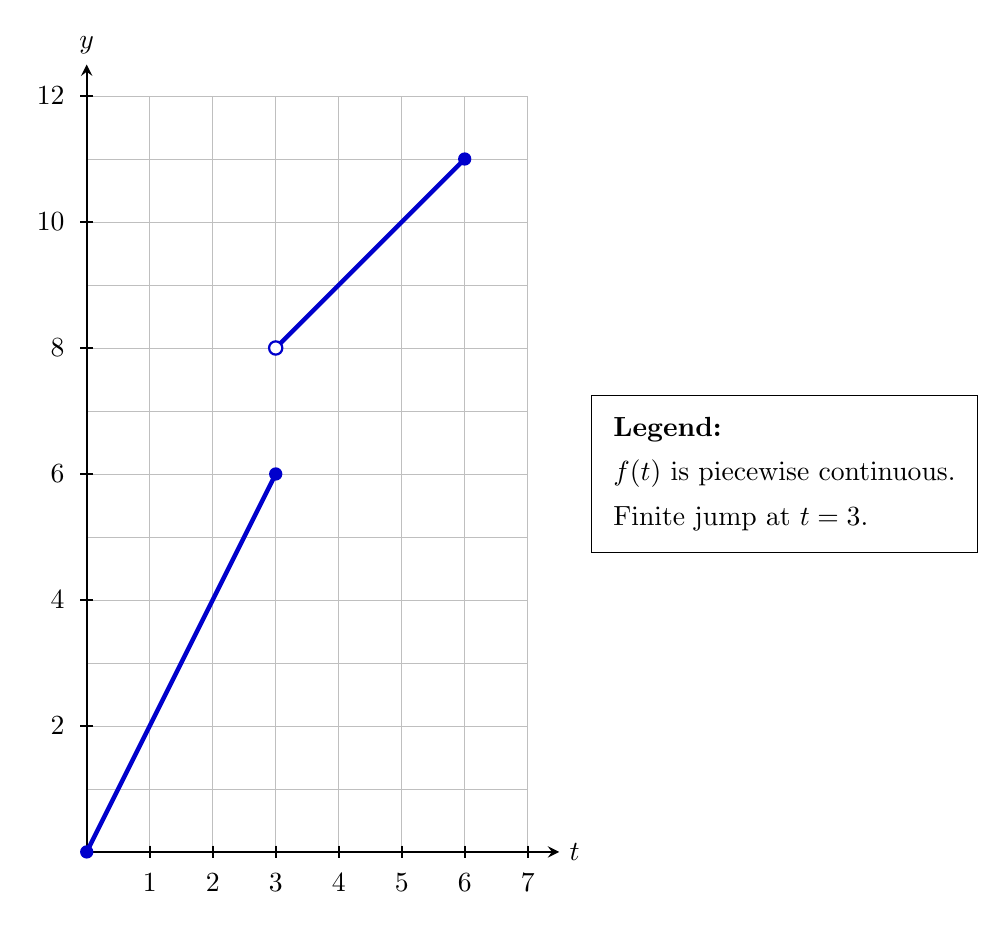
\begin{tikzpicture}[scale=0.8]
        % Background/Grid
        \draw[lightgray, very thin, step=1] (0,0) grid (7, 12);
        % Axes
        \draw[thick, ->, >=stealth] (0,0) -- (7.5,0) node[right] {$t$};
        \draw[thick, ->, >=stealth] (0,0) -- (0,12.5) node[above] {$y$};
        % Ticks
        \foreach \x in {1,...,7} \draw[thick] (\x, 0.1) -- (\x, -0.1) node[below=2pt] {$\x$};
        \foreach \y in {2,4,6,8,10,12} \draw[thick] (0.1, \y) -- (-0.1, \y) node[left=2pt] {$\y$};
        
        % Plots
        \draw[ultra thick, blue!80!black, domain=0:3, samples=50] plot (\x, {2*\x});
        \draw[ultra thick, blue!80!black, domain=3:6, samples=50] plot (\x, {\x + 5});
        
        % Discontinuity markers
        \fill[blue!80!black] (0,0) circle (3pt);
        \fill[blue!80!black] (3,6) circle (3pt);
        \draw[blue!80!black, thick, fill=white] (3,8) circle (3pt);
        \fill[blue!80!black] (6,11) circle (3pt);
        
        % Legend
        \node[align=left, draw, inner sep=8pt, anchor=west, fill=white] at (8, 6) {
            \textbf{Legend:}\\[4pt]
            $f(t)$ is piecewise continuous.\\[4pt]
            Finite jump at $t = 3$.
        };
    \end{tikzpicture}
    \end{center}

    % Solution 5
    \item \textbf{Statement:} Determine if $f(t) = \frac{1}{t-4}$ is piecewise continuous on $[0, 5]$.\\
    \textbf{Solution:} We analyze the behavior at $t = 4$. 
    \[
    \lim_{t \to 4^-} \frac{1}{t-4} = -\infty \quad \text{and} \quad \lim_{t \to 4^+} \frac{1}{t-4} = \infty
    \]
    Because the limits are infinite, this is an infinite (vertical asymptote) discontinuity, not a finite jump. \\
    \textbf{Final Answer:} The function is \textbf{neither} continuous nor piecewise continuous on $[0, 5]$.

    % Solution 6
    \item \textbf{Statement:} Determine if $f(t) = \frac{\sin(3t)}{t}$ is piecewise continuous on $[0, 10]$.\\
    \textbf{Solution:} We analyze the behavior at $t = 0$. Using the fundamental trigonometric limit:
    \[
    \lim_{t \to 0} \frac{\sin(3t)}{t} = \lim_{t \to 0} 3 \left( \frac{\sin(3t)}{3t} \right) = 3(1) = 3
    \]
    The function is explicitly defined as $f(0) = 0$. Since the limit exists and is finite ($3$), but does not equal the function value ($0$), there is a removable discontinuity at $t = 0$. Because the discontinuity is finite, it satisfies the definition.\\
    \textbf{Final Answer:} The function is \textbf{piecewise continuous}.

    % Solution 7
    \item \textbf{Statement:} Is $f(t) = e^{t^3}$ of exponential order?\\
    \textbf{Solution:} A function is of exponential order if $|f(t)| \le M e^{ct}$ for some constants $M, c > 0$ as $t \to \infty$. We compare growth rates:
    \[
    \lim_{t \to \infty} \frac{e^{t^3}}{e^{ct}} = \lim_{t \to \infty} e^{t^3 - ct} = \infty
    \]
    Because $t^3$ grows strictly faster than any linear term $ct$, the function cannot be bounded by a standard exponential.\\
    \textbf{Final Answer:} \textbf{No}, it is not of exponential order.

    % Solution 8
    \item \textbf{Statement:} Is $f(t) = t^4 \cos(2t)$ of exponential order?\\
    \textbf{Solution:} We know that $|\cos(2t)| \le 1$ for all $t$. Therefore, $|t^4 \cos(2t)| \le t^4$. Polynomials grow strictly slower than exponential functions, meaning $t^4 \le M e^{ct}$ for any $c > 0$ and sufficiently large $t$.\\
    \textbf{Final Answer:} \textbf{Yes}, it is of exponential order.

    % Solution 9
    \item \textbf{Statement:} Is $f(t) = \sinh(4t)$ of exponential order?\\
    \textbf{Solution:} By definition, $\sinh(4t) = \frac{e^{4t} - e^{-4t}}{2}$. For $t > 0$, this is strictly less than $\frac{1}{2}e^{4t}$. This perfectly matches the form $M e^{ct}$ with $M = 0.5$ and $c = 4$.\\
    \textbf{Final Answer:} \textbf{Yes}, it is of exponential order.

    % Solution 10
    \item \textbf{Statement:} Is $f(t) = e^{\frac{t^2+3}{t+2}}$ of exponential order?\\
    \textbf{Solution:} We perform polynomial long division on the exponent:
    \[
    \frac{t^2+3}{t+2} = t - 2 + \frac{7}{t+2}
    \]
    For $t \ge 0$, the fractional term $\frac{7}{t+2}$ is bounded by $\frac{7}{2} = 3.5$. Thus:
    \[
    f(t) = e^{t - 2 + \frac{7}{t+2}} \le e^{t - 2 + 3.5} = e^{1.5} e^t
    \]
    This is exactly in the form $M e^{ct}$ with $M = e^{1.5}$ and $c = 1$.\\
    \textbf{Final Answer:} \textbf{Yes}, it is of exponential order.

    % Solution 11
    \item \textbf{Statement:} Find $\mathscr{L}\{3t^4 - 5t^2 + 8\}$.\\
    \textbf{Solution:} Apply linearity and standard table formulas ($\mathscr{L}\{t^n\} = \frac{n!}{s^{n+1}}$):
    \[
    3\mathscr{L}\{t^4\} - 5\mathscr{L}\{t^2\} + 8\mathscr{L}\{1\} = 3\left(\frac{4!}{s^5}\right) - 5\left(\frac{2!}{s^3}\right) + 8\left(\frac{1}{s}\right)
    \]
    \textbf{Final Answer:} $F(s) = \frac{72}{s^5} - \frac{10}{s^3} + \frac{8}{s}$, defined for $s > 0$.

    % Solution 12
    \item \textbf{Statement:} Find $\mathscr{L}\{7\sin(3t) - 2\cos(5t)\}$.\\
    \textbf{Solution:} Apply linearity and standard table formulas:
    \[
    7\mathscr{L}\{\sin(3t)\} - 2\mathscr{L}\{\cos(5t)\} = 7\left(\frac{3}{s^2 + 9}\right) - 2\left(\frac{s}{s^2 + 25}\right)
    \]
    \textbf{Final Answer:} $F(s) = \frac{21}{s^2 + 9} - \frac{2s}{s^2 + 25}$, defined for $s > 0$.

    % Solution 13
    \item \textbf{Statement:} Find $\mathscr{L}\{(2t-1)^2\}$.\\
    \textbf{Solution:} First, expand the polynomial: $(2t-1)^2 = 4t^2 - 4t + 1$. Then apply linearity:
    \[
    4\mathscr{L}\{t^2\} - 4\mathscr{L}\{t\} + \mathscr{L}\{1\} = 4\left(\frac{2}{s^3}\right) - 4\left(\frac{1}{s^2}\right) + \frac{1}{s}
    \]
    \textbf{Final Answer:} $F(s) = \frac{8}{s^3} - \frac{4}{s^2} + \frac{1}{s}$, defined for $s > 0$.

    % Solution 14
    \item \textbf{Statement:} Find $\mathscr{L}\{4e^{6t} + 3e^{-2t}\}$.\\
    \textbf{Solution:} Apply linearity and the exponential rule ($\mathscr{L}\{e^{at}\} = \frac{1}{s-a}$):
    \[
    4\left(\frac{1}{s-6}\right) + 3\left(\frac{1}{s - (-2)}\right)
    \]
    The restrictions are $s > 6$ and $s > -2$. The intersection is $s > 6$.\\
    \textbf{Final Answer:} $F(s) = \frac{4}{s-6} + \frac{3}{s+2}$, defined for $s > 6$.

    % Solution 15
    \item \textbf{Statement:} Find $\mathscr{L}\{e^{-4t}t^3\}$.\\
    \textbf{Solution:} Use the First Translation Theorem. The base function is $f(t) = t^3$, so $F(s) = \frac{3!}{s^4} = \frac{6}{s^4}$ (for $s > 0$). The exponential shift is $a = -4$. We shift $s \to s - (-4) = s + 4$:
    \[
    F(s+4) = \frac{6}{(s+4)^4}
    \]
    The domain shifts from $s > 0$ to $s+4 > 0 \implies s > -4$.\\
    \textbf{Final Answer:} $F(s) = \frac{6}{(s+4)^4}$, defined for $s > -4$.

    % Solution 16
    \item \textbf{Statement:} Find $\mathscr{L}\{e^{2t}\cos(4t)\}$.\\
    \textbf{Solution:} The base function is $\cos(4t)$, so $F(s) = \frac{s}{s^2 + 16}$ (for $s > 0$). The shift is $a = 2$. We shift $s \to s - 2$:
    \[
    F(s-2) = \frac{s-2}{(s-2)^2 + 16}
    \]
    \textbf{Final Answer:} $F(s) = \frac{s-2}{(s-2)^2 + 16}$, defined for $s > 2$.

    % Solution 17
    \item \textbf{Statement:} Find $\mathscr{L}\{e^{-3t}\sin(5t) - e^{t}t^2\}$.\\
    \textbf{Solution:} Evaluate each term using the shift theorem:
    \begin{itemize}
        \item $\mathscr{L}\{e^{-3t}\sin(5t)\}$: Base $\sin(5t) \implies \frac{5}{s^2+25}$. Shift $s \to s+3 \implies \frac{5}{(s+3)^2+25}$, $s > -3$.
        \item $\mathscr{L}\{e^{t}t^2\}$: Base $t^2 \implies \frac{2}{s^3}$. Shift $s \to s-1 \implies \frac{2}{(s-1)^3}$, $s > 1$.
    \end{itemize}
    Combining them yields the final function. The intersection of $s > -3$ and $s > 1$ is $s > 1$.\\
    \textbf{Final Answer:} $F(s) = \frac{5}{(s+3)^2+25} - \frac{2}{(s-1)^3}$, defined for $s > 1$.

    % Solution 18
    \item \textbf{Statement:} Find $\mathscr{L}\{t^5 e^{-t}\}$.\\
    \textbf{Solution:} The base function is $t^5$, so $F(s) = \frac{5!}{s^6} = \frac{120}{s^6}$. The shift is $a = -1$, so $s \to s+1$.\\
    \textbf{Final Answer:} $F(s) = \frac{120}{(s+1)^6}$, defined for $s > -1$.

    % Solution 19
    \item \textbf{Statement:} Determine the domain restriction for $\mathscr{L}\{e^{5t} - e^{-2t} + t^3\}$.\\
    \textbf{Solution:} Find the restriction for each individual term:
    \begin{itemize}
        \item $\mathscr{L}\{e^{5t}\} \implies s > 5$
        \item $\mathscr{L}\{e^{-2t}\} \implies s > -2$
        \item $\mathscr{L}\{t^3\} \implies s > 0$
    \end{itemize}
    The overall domain is the intersection of all individual domains. The most restrictive condition is $s > 5$.\\
    \textbf{Final Answer:} The domain restriction is $s > 5$.

    % Solution 20
    \item \textbf{Statement:} Determine the domain restriction for $\mathscr{L}\{e^{3t}\cos(t) + e^{7t}\}$.\\
    \textbf{Solution:} Find the restriction for each individual term:
    \begin{itemize}
        \item $\mathscr{L}\{e^{3t}\cos(t)\} \implies s > 3$
        \item $\mathscr{L}\{e^{7t}\} \implies s > 7$
    \end{itemize}
    The intersection of $s > 3$ and $s > 7$ is $s > 7$.\\
    \textbf{Final Answer:} The domain restriction is $s > 7$.

    % Solution 21
    \item \textbf{Statement:} Find $\mathscr{L}\{y''\}$ if $y(0) = 3$ and $y'(0) = -1$.\\
    \textbf{Solution:} Use the Transform of a Derivative theorem:
    \[
    \mathscr{L}\{y''\} = s^2 Y(s) - sy(0) - y'(0)
    \]
    Substitute the initial conditions:
    \[
    \mathscr{L}\{y''\} = s^2 Y(s) - s(3) - (-1) = s^2 Y(s) - 3s + 1
    \]
    \textbf{Final Answer:} $\mathscr{L}\{y''\} = s^2 Y(s) - 3s + 1$.

    % Solution 22
    \item \textbf{Statement:} Find $\mathscr{L}\{y'\}$ if $y(0) = 5$.\\
    \textbf{Solution:} Use the Transform of a Derivative theorem:
    \[
    \mathscr{L}\{y'\} = s Y(s) - y(0) = s Y(s) - 5
    \]
    \textbf{Final Answer:} $\mathscr{L}\{y'\} = s Y(s) - 5$.

    % Solution 23
    \item \textbf{Statement:} Verify the derivative theorem for $f(t) = t^3$.\\
    \textbf{Solution:} First, compute the derivative manually: $f'(t) = 3t^2$. Using the table, $\mathscr{L}\{3t^2\} = 3\left(\frac{2}{s^3}\right) = \frac{6}{s^3}$.\\
    Next, use the theorem: $\mathscr{L}\{f'(t)\} = sF(s) - f(0)$. We know $F(s) = \mathscr{L}\{t^3\} = \frac{6}{s^4}$ and $f(0) = 0^3 = 0$.
    \[
    s\left(\frac{6}{s^4}\right) - 0 = \frac{6}{s^3}
    \]
    \textbf{Final Answer:} Both methods yield $\frac{6}{s^3}$, verifying the theorem.

    % Solution 24
    \item \textbf{Statement:} Find $\mathscr{L}\{(t-4)^2 \mathcal{U}(t-4)\}$.\\
    \textbf{Solution:} Use the Second Translation Theorem: $\mathscr{L}\{f(t-a)\mathcal{U}(t-a)\} = e^{-as}F(s)$. Here, $a = 4$ and the shifted function is $f(t-4) = (t-4)^2$, meaning the base function is $f(t) = t^2$. The transform of the base function is $F(s) = \frac{2}{s^3}$.\\
    \textbf{Final Answer:} $F(s) = e^{-4s} \frac{2}{s^3}$.

    % Solution 25
    \item \textbf{Statement:} Find $\mathscr{L}\{e^{3(t-2)} \mathcal{U}(t-2)\}$.\\
    \textbf{Solution:} Here, $a = 2$ and $f(t-2) = e^{3(t-2)}$, meaning the base function is $f(t) = e^{3t}$. The transform of the base function is $F(s) = \frac{1}{s-3}$.\\
    \textbf{Final Answer:} $F(s) = e^{-2s} \frac{1}{s-3}$.

    % Solution 26
    \item \textbf{Statement:} Find $\mathscr{L}\{\cos(t-\pi) \mathcal{U}(t-\pi)\}$.\\
    \textbf{Solution:} Here, $a = \pi$ and $f(t-\pi) = \cos(t-\pi)$, meaning the base function is $f(t) = \cos(t)$. The transform of the base function is $F(s) = \frac{s}{s^2+1}$.\\
    \textbf{Final Answer:} $F(s) = e^{-\pi s} \frac{s}{s^2+1}$.

    % Solution 27
    \item \textbf{Statement:} Find the flaw: $\mathscr{L}\{t \sin(2t)\} = \mathscr{L}\{t\} \cdot \mathscr{L}\{\sin(2t)\} = \frac{1}{s^2} \cdot \frac{2}{s^2+4}$.\\
    \textbf{Solution:} 
    \begin{itemize}
        \item \textbf{The Flaw:} The Laplace transform is a linear operator, but it does NOT distribute over multiplication; $\mathscr{L}\{f \cdot g\} \neq \mathscr{L}\{f\} \cdot \mathscr{L}\{g\}$.
        \item \textbf{The Correction:} You must use the derivative of a transform theorem: $\mathscr{L}\{t^n f(t)\} = (-1)^n \frac{d^n}{ds^n} F(s)$. Here, $n=1$ and $F(s) = \frac{2}{s^2+4}$.
        \[
        (-1)^1 \frac{d}{ds} \left( 2(s^2+4)^{-1} \right) = -1 \left( -2(s^2+4)^{-2}(2s) \right) = \frac{4s}{(s^2+4)^2}
        \]
    \end{itemize}

    % Solution 28
    \item \textbf{Statement:} Find the flaw: $\mathscr{L}\{e^{-6t} t^3\} \implies F(s-6) = \frac{6}{(s-6)^4}$.\\
    \textbf{Solution:}
    \begin{itemize}
        \item \textbf{The Flaw:} A sign error was made when applying the shift theorem. The formula is $s \to s - a$. Since $a = -6$, the shift becomes $s - (-6) = s + 6$.
        \item \textbf{The Correction:} The correct shift is $s + 6$, yielding $\frac{6}{(s+6)^4}$.
    \end{itemize}

    % Solution 29
    \item \textbf{Statement:} Find the flaw: Domain for $\mathscr{L}\{e^{4t} + e^{8t}\}$ is $s > 4 \cup s > 8 \implies s > 4$.\\
    \textbf{Solution:}
    \begin{itemize}
        \item \textbf{The Flaw:} The combined domain must be the \textit{intersection} (the most restrictive condition), not the union, because both integrals must converge simultaneously.
        \item \textbf{The Correction:} The intersection of $s > 4$ and $s > 8$ is $s > 8$.
    \end{itemize}

    % Solution 30
    \item \textbf{Statement:} Find the flaw: $f(t) = e^{t^5}$ is of exponential order because it is an exponential function.\\
    \textbf{Solution:}
    \begin{itemize}
        \item \textbf{The Flaw:} A fundamental misunderstanding of "exponential order". The function must be bounded by $e^{ct}$ for a constant $c$, but $t^5$ grows faster than $ct$.
        \item \textbf{The Correction:} No, it is not of exponential order because $\lim_{t \to \infty} \frac{e^{t^5}}{e^{ct}} = \infty$ for any constant $c$.
    \end{itemize}

\end{enumerate}

\end{document}